\documentclass{beamer}
\usetheme{default}

\usepackage{subfigure}
\usepackage{amsmath}
\usepackage{gensymb}

\begin{document}

\begin{frame}{}

\title{\textbf{Image Processing}}
\maketitle

Chloe Eghtebas, Luke Metz, Brendan Ritter

\end{frame}


\begin{frame}{Basics of Image Processing}

\begin{figure}
\includegraphics[width = 1.5 in]{cool.jpg}
\hspace{1.5 in}
\includegraphics[width = 1 in]{brain.jpg}
\end{figure}

Using computational software to manipulate an image using signal processing techniques. 

\hspace{0.25 in}
\includegraphics[width = 1.5 in]{satilite.jpg}
\hspace{1 in}
\includegraphics[width = 1 in]{forensic}

\end{frame}



\begin{frame}{What You'll Learn}

\begin{itemize}
		
	\item[1]"Signal Processing" 
	\item Shear
    \item brightness and contrast 
    \item grayscale
    \item invert
    \item Rotating
    	\item Flipping
    \item[2]Edge Detection 
    \item Gaussian blur
    \item Sobel/convolution
\end{itemize}
\end{frame}

\begin{frame}{Image Representation and Software}

\begin{figure}
\begin{center}
\includegraphics[width = 0.75 in]{bunny.jpg}
\end{center}
\end{figure}

Images have 3 channels. Red, Blue, Green. To manipulate these arrays we chose to not use matlab. We chose to use Python and Numpy mainly for its re usability.

\begin{figure}
\includegraphics[width = 0.75 in]{bunnyred.png}
\hspace{0.5 in}
\includegraphics[width = 0.75 in]{bunnygreen.png}
\hspace{0.5 in}
\includegraphics[width = 0.75 in]{bunnyblue.png}
\end{figure}

\end{frame} 


\begin{frame}{Flipping}
To flip our images, we took our 3 large matrices, rgb, and multiplied them by a matrix like the one bellow except the right size.
$A = \begin{pmatrix}
	0 & 0 & 0 & 1\\
	0 & 0 & 1 & 0\\
	0 & 1 & 0 & 0\\
	1 & 0 & 0 & 0\\
\end{pmatrix}$
To flip horizontally, one can multiply $AI$. To flip vertically, one can $IA$.

\begin{figure}
\includegraphics[width = 0.9 in]{lennastory.jpg}
\hspace{0.5 in}
\includegraphics[width = 0.9 in]{lenna1.png}
\hspace{0.5 in}
\includegraphics[width = 0.9 in]{lenna2.png}
\caption{Original Image, flipped vertically, flipped horizontally.}
\end{figure}


\end{frame}


\begin{frame}{Transformations}
To apply more complicated transformations to the image one first has to re arrange the image. Currently x and y position are stored at the index of the matrix. This gives us no easy way to manipulate them.

We can rearrange The image to look like:
$$A = \begin{pmatrix}
	x & 0 & 1 &...\\
	y & 0 & 0 &...\\
	1 & 1 &  1 &...\\
	r &  255 & 255 &...\\
	g & 255 & 255 &...\\
	b & 255 & 255 &...\\
\end{pmatrix}$$
This will let us translate, rotate, scale, and shear the image in any way.

\end{frame}

\begin{frame}{Rotation}
Example Rotation:
The Default rotation is always around the origin. To make that the center of the image, one must first translate, rotate, then translate back.
\hspace{0.1 in}
\\
$A_{out} = \begin{pmatrix}
	1 & 0 & dx\\
	0 & 1 & dy\\
	0 & 0 & 1\\
\end{pmatrix}$
$\begin{pmatrix}
	\cos(\theta) & -\sin(\theta) & 0\\
	\sin(\theta)& \cos(\theta) & 0\\
	0 & 0 & 1\\
\end{pmatrix}$
$\begin{pmatrix}
	1 & 0 & -dx\\
	0 & 1 & -dy\\
	0 & 0 & 1\\
\end{pmatrix}$
$A$
\\
\begin{figure}


\includegraphics[width = 1.1 in]{bunnycute.jpg}
\hspace{0.5 in}
\includegraphics[width = 1.1 in]{bunnycuteRot.jpg}
\caption{Rotated around the center at $\theta = 45\degree$}
\end{figure}
\end{frame}


\begin{frame}{Shear}
Example Shear:

\hspace{0.1 in}
\\
$A_{out} = \begin{pmatrix}
	1 & \lambda_y & 0\\
	\lambda_x & 1 & 0\\
	0 & 0 & 1\\
\end{pmatrix}$
$A$
\\
\begin{figure}

\includegraphics[width = 1.1 in]{bunnycute.jpg}
\hspace{0.5 in}
\includegraphics[width = 1.1 in]{bunnycuteShear.jpg}
\caption{Sheared with $\lambda_X = .4$ and $\lambda_Y = 0$}
\end{figure}

\end{frame}


\begin{frame}{Color}
Our next feature that we implemented was color controls per channel. This would let us control how much of one color there is as well as increase or decreases brightness, changing all channels. This can be done by simply adding values to the matrix at each channel.

\begin{figure}[ht]
\includegraphics[width=1.4in]{parrot.jpg}
\hspace{.1in} 
\includegraphics[width=1.4in]{parrotout1.jpg}
\hspace{.1in}
\includegraphics[width=1.4in]{parrotout2.jpg}
\hspace{.1in}
\caption{In order from left to right, original image, red increased with green and blue decreased, all channels decreased.}
\end{figure}
\end{frame}

\begin{frame}{Convolution}

Convolution is apply‌g one function to another to construct an output of the system. 
\newline

\begin{figure}
\begin{center}
\includegraphics[width= 1.4 in]{convolution.png}
\end{center}
\end{figure}
Same priciple for discreate convolution. It's like overlapping one signal with another. One signal has original data and is convolved with a kernel which represents the other function. 


\end{frame}

\begin{frame} {Convolution in 1d}
In 1d, one can think of super imposing the kernel over each point ofl data.
$$A = (0,2,3,1,2,1,0)$$
$$K = (1,1,1)$$ 
$$O = A*K = (2,5,6,6,4,3,1)$$

Or Mathematically for a kernel of size 3, $O_n = A_{n-1}*K_{0}+A_{n}*K_{1}+A_{n+1}*K_{2}$

Because our vectors are not infinite, we have to decide what happens on the edges. We will assume that the $A_{-1} = A_{n-1}$ where n is the size of the vector.
\end{frame}


\begin{frame}{Multiplying Matrices}
Convolution around a kernel is a linear operator, thus one can find a matrix, $C$, that transforms A to O. $CA=O=A*K$.

$C = \begin{pmatrix}
	1 & 1 & 0 & 0 & 0 & 0 & 1\\
	1 & 1 & 1 & 0 & 0 & 0 & 0\\
	0 & 1 & 1 & 1 & 0 & 0 & 0\\
	0 & 0 & 1 & 1 & 1 & 0 & 0\\
	0 & 0 & 0 & 1 & 1 & 1 & 0\\
	0 & 0 & 0 & 0 & 1 & 1 & 1\\
	1 & 0 & 0 & 0 & 0 & 1 & 1\\
\end{pmatrix}$

This matrix is in the form of a Circulant matrix. Matrices in this form are easy to analyze.

\end{frame}


\begin{frame}{Eigen Things}
Because this matrix is Circulant, its eigen vectors and values are easy to find. 
Assuming the following circulant matrix, 
$$\begin{matrix}
	c_0 & c_{n-1} & \cdots & c_2 & c_1\\
	c_1 & c_0 & c_{n-1} &  & c_2\\
	\vdots & c_1 & c_0 & \ddots & \vdots\\
	c_{n-2} &   & \ddots & \ddots & c_{n-1}\\
	c_{n-1} & c_{n-2} & \cdots & c_1 & c_0\\
\end{matrix}$$
The eigen values and vectors are:
$$\lambda_j =c_0+c_{n-1}w_j	+c_{n-2}w_j^2+...+c_{1}w_j{n-1}2$$
$$v_j = (1, w_j, w_j^2, w_j^3, ..., w_j^{n-1})$$

Where $w$ are the roots of unity, $z^n = 1$ or 
$$w_j = e^{\dfrac{2\pi i j}{n}}$$

\end{frame}

\begin{frame}{Eigen Things, cont}
For our demo kernel,
$$\lambda_j = 1+e^{\dfrac{2\pi i j}{n}}+e^{\dfrac{(n-1)\pi i j}{n}}$$

we can say $(n-1) = -1$ to simplify because we multiplying by $2\pi$. Thus   
$$\lambda_j = 1+e^{\dfrac{2\pi i j}{n}}+e^{\dfrac{-\pi i j}{n}}$$
Using eulers formula
$$\lambda_j = 1+2\cos(\dfrac{2\pi j}{n})$$
$$\lambda_{0} = 3$$ is the maximum eigen value.
This value corresponds to $v_0 = (1,1,1,1,1...)$.
Take for example $\lambda_{n/2} = -1$.  $v_{n/2} = (1,-1,-1,1,-1...)$.

\end{frame}

\begin{frame}{What this Means?}
One can look at this filter and see that it is a form of blur. It takes the two values next to a point and adds them.  This also multiplies the magnitude of the list by 3, hence an eigen value of 3. This eigen value coresponds to a very low frequency. The smallest eigen values, $\lambda_{n/2} = -1$ corresponds to the highest frequency. The blur is passing through low frequencies and reducing high frequencies.
\end{frame}

\begin{frame}{Convolution in 2d}
One can extend the above by thinking about an image as a flat vector. This makes it quite hard to think about kernels that act in both x and y. This is why 2d convolution makes a lot of sense.
\begin{figure}[htp]
\centering
\includegraphics[width=2in]{conv2d_matrix.jpg}
\caption{Convolution in 2D.}
\label{}
\end{figure}
Doing this allows for a much more concise way to write down convolution kernels.
\end{frame}


\begin{frame}{Gaussian Blur}

Gaussian blur is an application of  convolution. It 'blends' a Gaussian, a normal curve onto the image. One has control over blurriness by the standard deviation, $\sigma$.

%\begin{figure}[ht]
%\begin{minipage}[b]{0.1\linewidth}
%\centering
%\includegraphics[width=1.3in]{churchin.jpg}
%\caption{Default Image}
%\label{fig:figure1}
%\end{minipage}
%\hspace{2.0in}
%\begin{minipage}[b]{0.1\linewidth}
%\centering
%\includegraphics[width=1.3in]{churchoutb.jpg}
%\caption{Blurred Image}
%\hspace{1.0in}
%\label{fig:figure2}
%\end{minipage}
%\end{figure}

\begin{figure}[ht]
\includegraphics[width=1.3in]{churchin.jpg}
\hspace{.1in}
\includegraphics[width=1.3in]{churchoutblur.jpg}
\hspace{.1in}
\includegraphics[width=1.3in]{churchoutblur2.jpg}
\caption{Original image on left. $\sigma$ = 2 in middle. $\sigma$ = 4 on left.}
\end{figure}
\end{frame}

\begin{frame}{Gaussian Function}
The Gaussian function in 2d is:
$$G(x,y) = \dfrac{1}{2\pi \sigma^2}e^{-\dfrac{x^2+y^2}{2 \sigma^2}}$$

In 1d it is:
$$ G(x) = \dfrac{1}{\sqrt{2\pi \sigma^2}}e^{\dfrac{-x^2}{2\sigma^2}}$$

\begin{figure}[ht]
\includegraphics[width=2.4in]{gauss.png}
\end{figure}
\end{frame}


\begin{frame} {Eigen values}
The eigenvalues of this Gaussian kernel preforms a form of bluring operation. Because of this, we know that its dominant eigen value is $\lambda_0$ which corresponds to a eigenvector which is low frequency. And it less dominant eigenvalues, $\lambda_{n/2}$ corresponds to high frequency.
\end{frame}


\begin{frame}{Sobel Edge Detection}
Another application of convolution is edge detection. The Sobel operator can be thought of as a discrete differentiation operator. It gets how fast one color goes to another. 

\begin{figure}[ht]
\includegraphics[width=1.4in]{edgein.png}
\hspace{.1in}
\includegraphics[width=1.4in]{edgeout.jpg}
\hspace{.1in}
\end{figure}
\end{frame}

\begin{frame}{Example}
\begin{figure}[ht]
\includegraphics[width=1.4in]{churchin.jpg}
\hspace{.1in}
\includegraphics[width=1.4in]{churchout.jpg}
\hspace{.1in}
\end{figure}
\end {frame}

\begin{frame}{Sobel Kernel}
The kernel used to create this edge detection is in two parts:\newline

$K_X = \begin{pmatrix}
	-1 & 0 & 1\\
	-2 & 0 & 2\\
	-1 & 0 & 1\\
\end{pmatrix}$
$K_Y = \begin{pmatrix}
	-1 & -2 & -1\\
	0 & 0 & 0\\
	1 & 2 & 1\\
\end{pmatrix}$\newline

Where $G_{x}$ is how quickly the colors change in the x direction and $G_{y}$ is in the y direction.
%\vspace{.4in}
\newline

$E = \sqrt(E_Y^2+E_Y^2)$ Where $E_X$ and $E_Y$ are the result of the convolution.
\end{frame}

\begin{frame}{Example of $G_{x}$ and $G_{y}$ Output}

After $G_{x}$ and $G_{y}$ are convolved with every element in the image matrix the output looks like:

\begin{figure}[ht]
\includegraphics[width= 1.4 in]{churchx.jpg}
\hspace{0.5 in}
\includegraphics[width= 1.4 in]{churchy.jpg}
\caption{$G_{x}$ and $G_{y}$ respectively}
\end{figure}

\end{frame}

\begin{frame}{Laplacian kernel}
A discrete Laplacian kernel can also be used to do edge detection. 
$K_L = \begin{pmatrix}
	-1 & -1 & -1\\
	-1 & 8 & -1\\
	-1 & -1 & -1\\
\end{pmatrix}$
\begin{figure}[ht]
\includegraphics[width=1.4in]{churchin.jpg}
\hspace{.1in}
\includegraphics[width=1.4in]{churchoutlaplace.jpg}
\hspace{.1in}
\end{figure}

\end{frame}

\begin{frame}{Blur + Edge Detection}
One can combine these operations to find the major edges in an image. Bellow are using Sobel edge detection.

\begin{figure}[ht]
\includegraphics[width=1.3in]{churchout.jpg}
\hspace{.1in} 
\includegraphics[width=1.3in]{churchoutbluredge.jpg}
\hspace{.1in}
\includegraphics[width=1.3in]{churchoutblur2edge.jpg}
\hspace{.1in}
\caption{No Blur, Blur, $\sigma = 2$, $\sigma = 4$}
\end{figure}
\end{frame}

\begin{frame}
Questions?
\end{frame}



\end{document}
